\section{Method}
\label{sec:method}

\begin{figure*}[t]
  \centering
  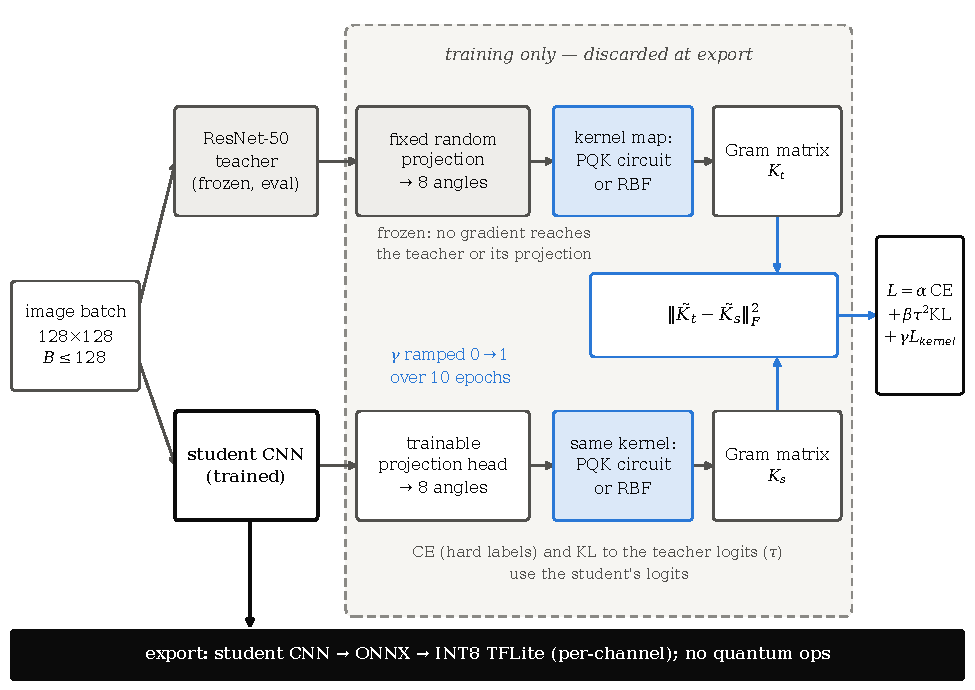
\includegraphics[width=\textwidth]{pipeline}
  \caption{Training-time pipeline. Penultimate features of the frozen teacher and of the student are projected to eight angles and compared through the Gram matrices of one kernel (the PQK circuit or an RBF kernel). Everything inside the dashed region is discarded at export; only the student CNN is deployed.}
  \label{fig:pipeline}
\end{figure*}

Let $x$ be an image with label $y$, let $z_t(x)\in\mathbb{R}^{2048}$ and $z_s(x)\in\mathbb{R}^{d_s}$ be the penultimate features of the teacher and the student, and let $\ell_t,\ell_s$ be their logits.
All losses are computed on batches of up to $B=128$ images; the last batch of an epoch is smaller, and the $33$-image RPS-25 validation split is a single batch.

\subsection{Baseline objectives}
\label{sec:objectives}

\Scratch minimizes the cross-entropy $\mathrm{CE}(\ell_s,y)$.
\Kd is Hinton distillation~\citep{hinton2015distilling},
\begin{equation}
  \begin{split}
  L_{\mathrm{KD}} ={}& \alpha\,\mathrm{CE}(\ell_s,y)\\
  &+ \beta\,\tau^{2}\,\mathrm{KL}\!\left(\mathrm{softmax}(\ell_t/\tau)\,\Vert\,\mathrm{softmax}(\ell_s/\tau)\right),
  \end{split}
\end{equation}
with $\alpha=\beta=0.5$ and a temperature $\tau$ that was screened on some pairs and reused on others (Table~\ref{tab:hparams-methods}).
\Rkd~\citep{park2019relational} adds distance-wise and angle-wise relational terms on the penultimate features,
\begin{equation}
  \begin{split}
  L_{\mathrm{RKD}} ={}& \mathrm{CE}(\ell_s,y) + w_d\,\mathrm{SmoothL1}\big(\psi_D(z_s),\psi_D(z_t)\big)\\
  &+ w_a\,\mathrm{SmoothL1}\big(\psi_A(z_s),\psi_A(z_t)\big),
  \end{split}
\end{equation}
where $\psi_D$ collects the pairwise distances of a batch normalized by their mean and $\psi_A$ the cosines of the angles formed by triplets.
Both potentials are dimension-free, so a 2048-dimensional teacher and a student of any width can be compared directly.

\subsection{Kernel alignment}
\label{sec:kernel-alignment}

The two kernel methods (\Pqk and its twin \Rbf) add a kernel-alignment term to the logit objective,
\begin{equation}
  L = \alpha\,\mathrm{CE}(\ell_s,y) + \beta\,\tau^{2}\,\mathrm{KL}(\cdot) + \gamma_e\,L_{\mathrm{kernel}},
  \label{eq:loss}
\end{equation}
\begin{equation}
  L_{\mathrm{kernel}} = \big\Vert \tilde K_t - \tilde K_s \big\Vert_F^{2},\qquad
  \tilde K = \frac{K}{\operatorname{tr}K},
\end{equation}
with $\alpha=\beta=0.5$, a single temperature $\tau=0.5$ for all kernel methods, and the weight $\gamma_e=\gamma_{\max}\min\!\big(1,(e{+}1)/10\big)$ ramped linearly over the first ten epochs $e$, with $\gamma_{\max}=1$.
Validation is always scored at $\gamma_{\max}$ so that the ramp cannot change which checkpoint is selected.
$K_t$ and $K_s$ are the $B\times B$ Gram matrices of the teacher and the student, built from eight angles per image,
\begin{equation}
  \theta_s = \pi\,\sigma(W_s z_s + b_s),\quad
  \theta_t = \pi\,\sigma(W_t z_t + b_t),\quad \theta\in[0,\pi]^{8}.
\end{equation}
The student-side projection $(W_s,b_s)$ is trained jointly with the student, and gradients reach the student through the kernel.
The teacher-side projection $(W_t,b_t)$ is drawn at default initialization at the start of each run, frozen, and evaluated without gradients.
Freezing it is necessary. If both projections are trainable, collapsing both to constant maps sets every Gram entry to one and makes the two normalized matrices identical. The loss $L_{\mathrm{kernel}}$ then reaches exactly zero without the student learning anything.
Our first implementation had this flaw. In the first \Pqk run we inspected (RPS-25, LeNet-5, seed~0) the mean off-diagonal kernel value was \CollapseStudent{} for the student and \CollapseTeacher{} for the teacher\extra{; Appendix~\ref{app:pitfalls} gives the details}.
We log the mean off-diagonal kernel value in every epoch and treat values below $0.05$ or above $0.95$ as degenerate.

\subsection{The projected quantum kernel}
\label{sec:pqk}

\begin{figure*}[t]
  \centering
  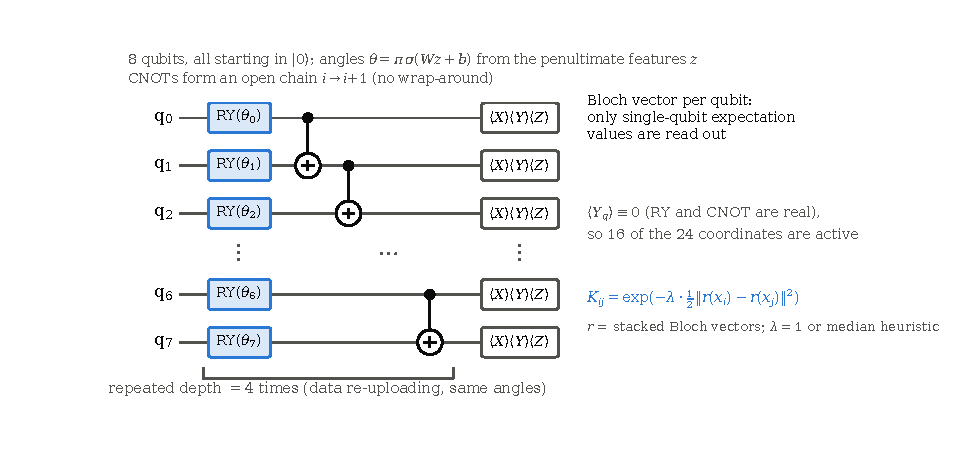
\includegraphics[width=\textwidth]{pqk_circuit}
  \caption{The fixed feature map behind \Pqk (shown for qubits $0$, $1$, $2$ and $7$). Each of the eight angles drives an $R_Y$ rotation, followed by an open chain of CNOT gates; the pair is repeated $4$ times with the same angles. Only single-qubit expectation values are read out. Nothing in the circuit is trainable.}
  \label{fig:circuit}
\end{figure*}

The quantum kernel is the projected quantum kernel of Huang et al.~\citep{huang2021power}.
The circuit (Figure~\ref{fig:circuit}) applies $R_Y(\theta_q)$ to every qubit $q$ and then a CNOT from qubit $q$ to $q{+}1$ for $q=0,\dots,6$, and repeats this pair of layers $4$ times on $8$ qubits starting from $|0\rangle^{\otimes 8}$.
The CNOTs form an open chain, with no gate closing it into a ring.
For each input the Bloch vector of every qubit is measured, $r(\theta)=(\langle X_q\rangle,\langle Y_q\rangle,\langle Z_q\rangle)_{q=0}^{7}$.
Because $R_Y$ and CNOT are real matrices, the state stays real and $\langle Y_q\rangle\equiv0$, so only $16$ of the $24$ coordinates are active.
The kernel compares inputs through their single-qubit reduced states $\rho_q=\tfrac12(I+r_q\cdot\sigma)$,
\begin{equation}
  \begin{split}
  K(\theta,\theta') &= \exp\!\Big(-\lambda\sum_{q}\big\Vert\rho_q(\theta)-\rho_q(\theta')\big\Vert_F^{2}\Big)\\
  &= \exp\!\Big(-\tfrac{\lambda}{2}\,\big\Vert r(\theta)-r(\theta')\big\Vert^{2}\Big),
  \end{split}
  \label{eq:pqk}
\end{equation}
where the second form follows from $\operatorname{tr}(\sigma_a\sigma_b)=2\delta_{ab}$.
The readout is restricted to single-qubit expectation values. At eight qubits the circuit is cheap to simulate exactly, so the kernel is classically tractable at this size. We use PennyLane~\citep{bergholm2018pennylane} on its state-vector \texttt{lightning.qubit} backend with adjoint differentiation.

The scale $\lambda$ is handled in two ways.
\Pqk uses the pre-specified $\lambda=1$.
The variant \texttt{pqk\_adaptive}, adopted after the first results (Section~\ref{sec:setup-protocol}), sets $\lambda$ in every batch so that $K=\exp\!\big(-d^{2}/(2m)\big)$ with $d^{2}=\tfrac12\Vert\Delta r\Vert^{2}$ and $m$ the median off-diagonal $d^{2}$ of the batch.
With this choice the Gram matrix is the median-heuristic RBF kernel on the measured features $r(\theta)$.

\subsection{Matched classical controls}
\label{sec:controls}

\Rbf is the same pipeline with an RBF kernel, $K=\exp\!\big(-\Vert\theta-\theta'\Vert^{2}/(2m)\big)$, on the same eight angles with the same median heuristic.
The quantum branch with adaptive $\lambda$ and \Rbf therefore differ only in the map $\theta\mapsto r(\theta)$ that precedes an identically calibrated RBF kernel.
Two further arms isolate where an effect of that map could come from.
\begin{itemize}
  \item \texttt{noent\_control} deletes the CNOT gates from the circuit.
  Each qubit then sees $R_Y(\theta_q)^{4}=R_Y(4\theta_q)$, so $r=(\sin4\theta_q,0,\cos4\theta_q)$ exactly (checked against the simulator to $6\times10^{-8}$), with the same $16$ active coordinates and range, no trainable parameters and the same adaptive RBF kernel. It differs from \texttt{pqk\_adaptive} only by entanglement.
  \item \texttt{pqk\_fit} and \texttt{rbf\_fit} replace the random teacher-side projection by a map fitted once on the training split and then frozen: the $C{-}1$ shrinkage-LDA directions, completed to eight outputs with the leading principal components of the residual and standardized on the training set.
\end{itemize}
A third control, random Fourier features drawn from the circuit's own frequency spectrum, was implemented but not run\extra{ (Section~\ref{sec:limitations})}.
Table~\ref{tab:kernel-cfg} lists the settings of every kernel arm.

\begin{table*}[t]
  \centering
  \caption{Kernel arms. All use eight angles, the loss of Eq.~\eqref{eq:loss} and the same frozen teacher.}
  \label{tab:kernel-cfg}
  \adjustbox{max width=\textwidth}{\begin{tabular}{@{}llrrll@{}}
\toprule
Method & Kernel on the 8 angles & Qubits & Depth & $\lambda$ / bandwidth & Teacher projection \\
\midrule
\texttt{rbf\_control} & RBF & 8 & -- & median heuristic & random (frozen) \\
\texttt{pqk} & projected quantum (RY+CNOT) & 8 & 4 & 1 & random (frozen) \\
\texttt{pqk\_adaptive} & projected quantum (RY+CNOT) & 8 & 4 & median heuristic & random (frozen) \\
\texttt{noent\_control} & classical map $[\sin4\theta,\cos4\theta]$ & 8 & 4 & median heuristic & random (frozen) \\
\texttt{pqk\_fit} & projected quantum (RY+CNOT) & 8 & 4 & median heuristic & LDA+PCA (fitted, frozen) \\
\texttt{rbf\_fit} & RBF & 8 & -- & median heuristic & LDA+PCA (fitted, frozen) \\
\bottomrule
\end{tabular}
}
\end{table*}

\subsection{What is trained and what is deployed}
\label{sec:deployed}

Only the student CNN is exported.
The projection heads, the circuit and the kernels exist only inside the training loop, and a purity check on the exported graph fails if any of them is present (Section~\ref{sec:setup-int8}).
The deployed model of every method, including \Pqk, is therefore an ordinary convolutional network, and the quantum kernel affects it only through the weights it learned.
